\section{Zeitmanagement}

\subsection{Zeitaufwand pro Person}

In der folgenden Grafik ist der Zeitaufwand pro Person für das ganze Projekt aufgezeigt.

\begin{figure}[H]
	\centering
	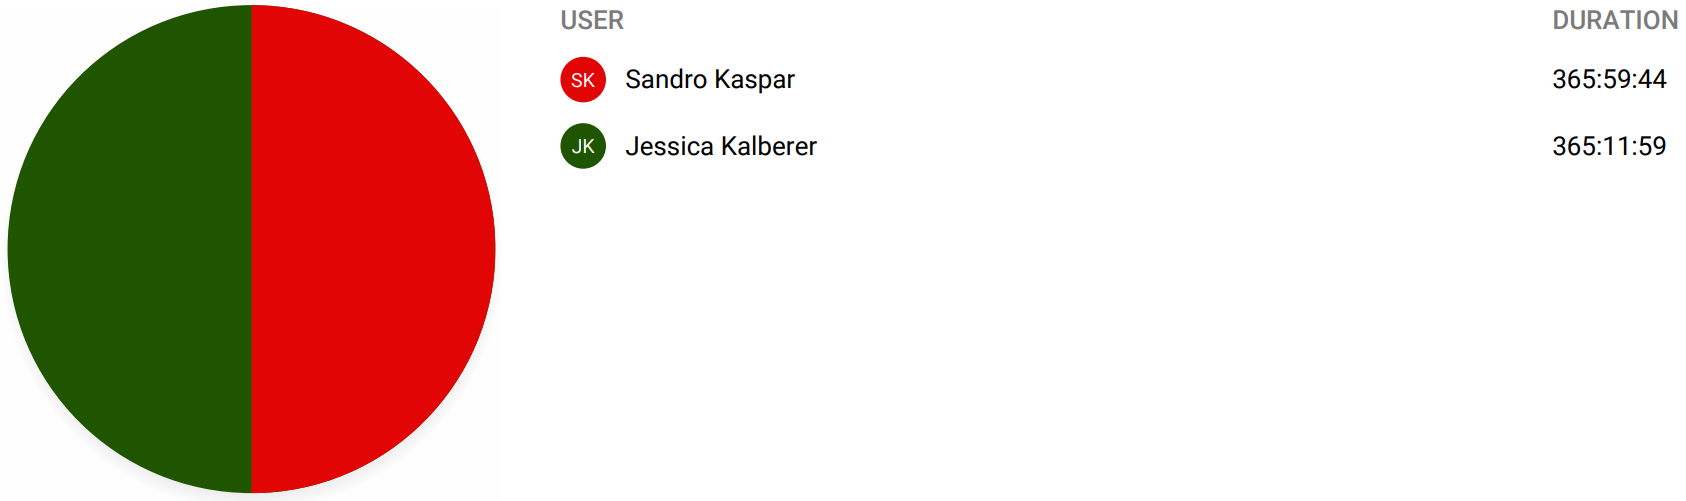
\includegraphics[width=1\linewidth]{img/Zeitmanagement/timeperuser}
	\caption{Zeitaufwand pro Person}
	\label{fig:Zeitaufwand pro Person}
\end{figure}




\subsection{Zeitaufwand pro Woche}
Der Zeitaufwand pro Woche ist in der nachfolgenden Grafik ersichtlich. Dabei ist zu erwähnen das in den letzten zwei Wochen frei genommen wurde, um die komplette Zeit in die Bachelorarbeit zu investieren.


\begin{figure}[H]
	\centering
	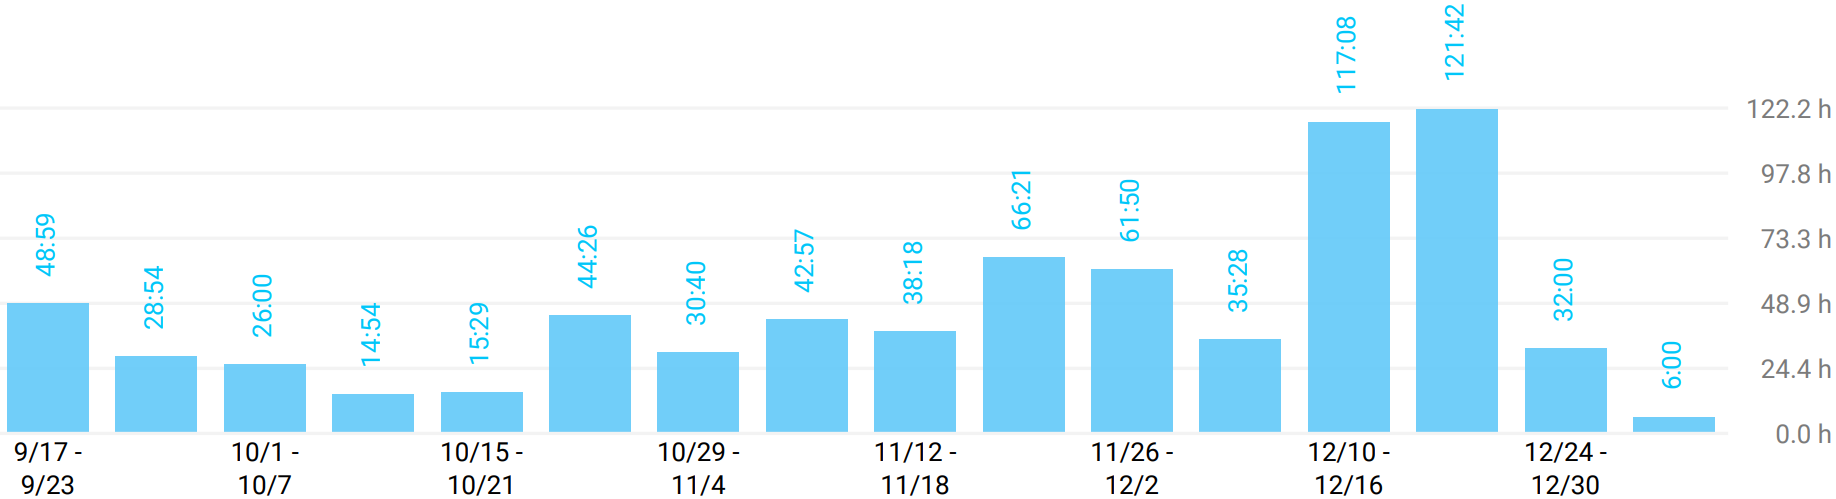
\includegraphics[width=1\linewidth]{img/Zeitmanagement/timeperweek}
	\caption{Zeitaufwand pro Woche}
	\label{fig:Zeitaufwand pro Woche}
\end{figure}




\subsection{Verteilung Zeitaufwand pro Issue}

Die nachfolgende Grafik beschreibt die Verteilung des Zeitaufwandes auf die einzelnen Issues.

\begin{figure}[H]
	\centering
	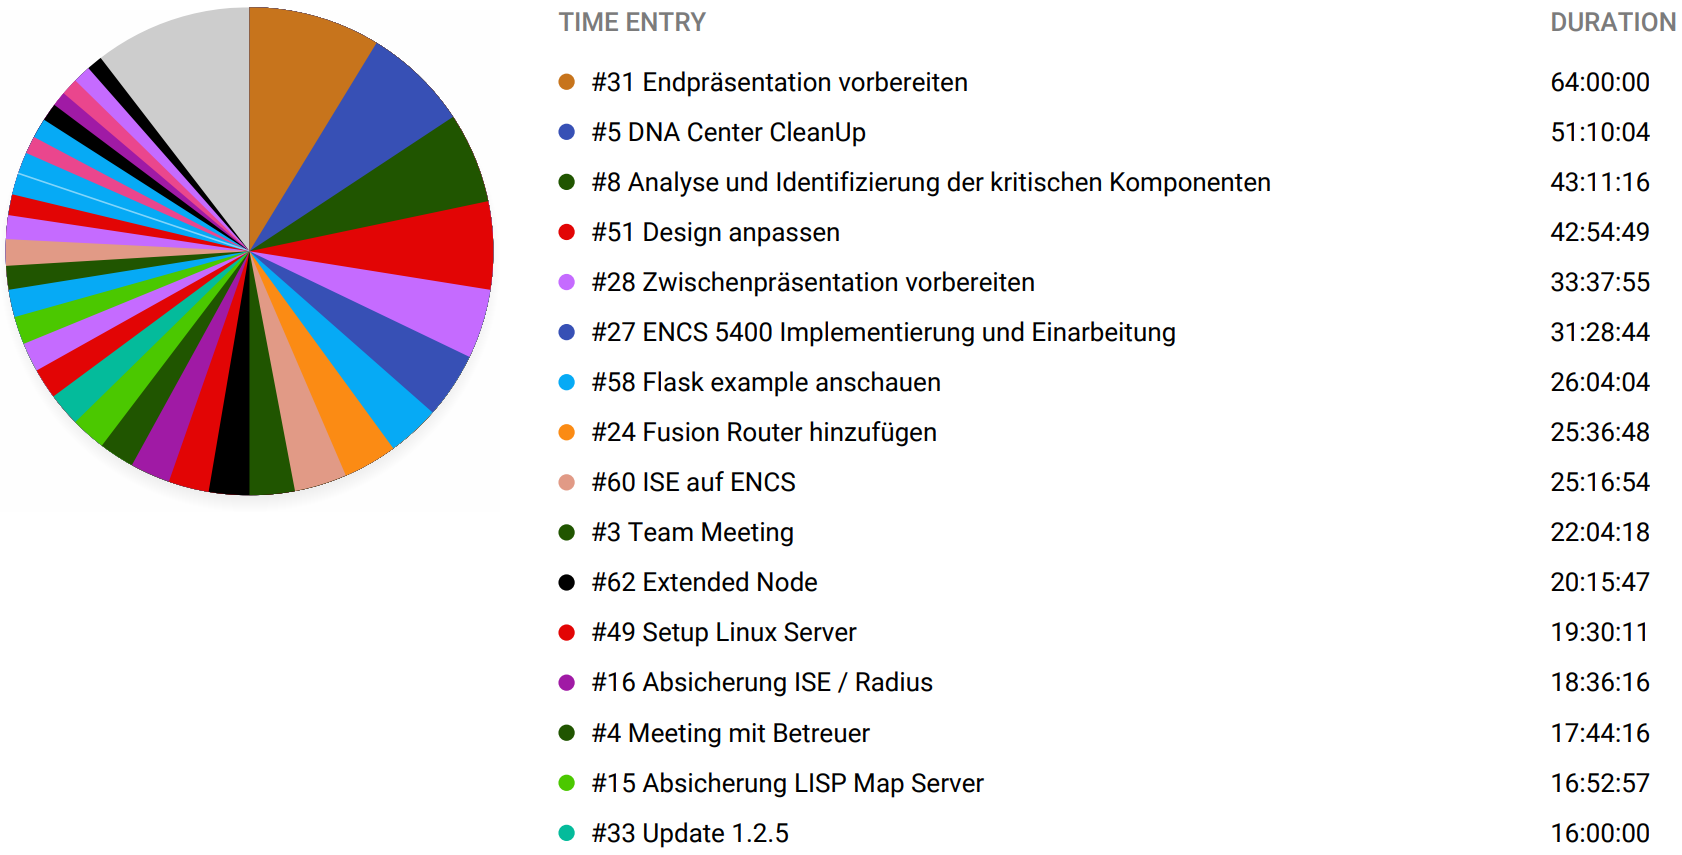
\includegraphics[width=1\linewidth]{img/Zeitmanagement/timeentry}
\end{figure}

\begin{figure}[H]
	\centering
	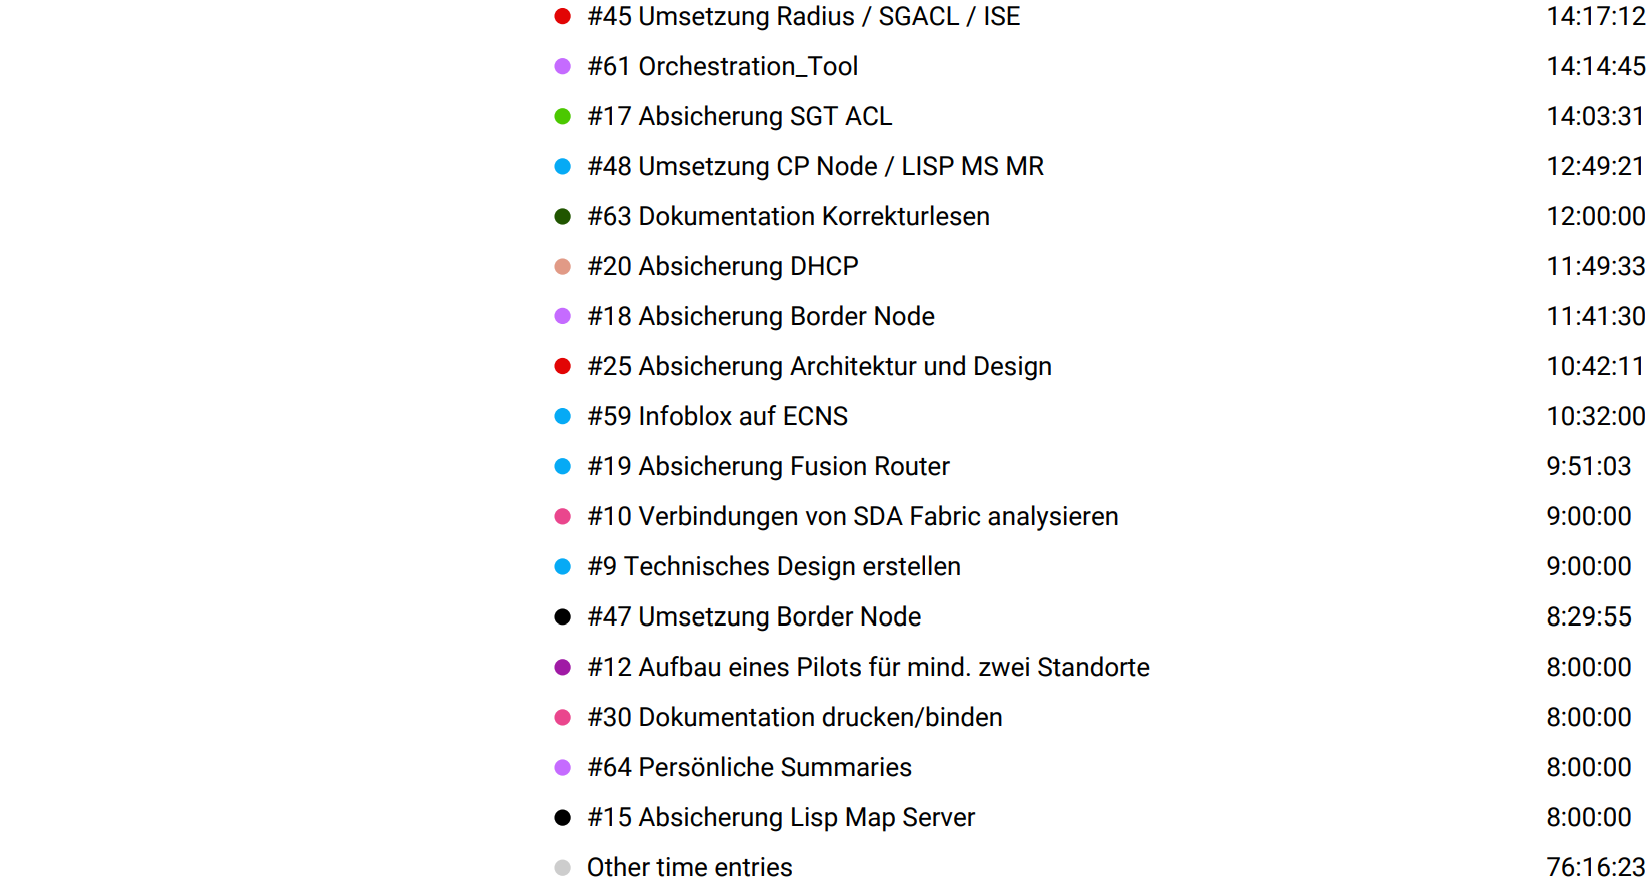
\includegraphics[width=1\linewidth]{img/Zeitmanagement/timeentry2}
	\caption{Verteilung Zeitaufwand pro Kategorie}
	\label{fig:Verteilung Zeitaufwand pro Kategorie}
\end{figure}